\documentclass{beamer}
\usetheme{Madrid}

\usepackage{amsmath, amssymb, amsthm}
\usepackage{graphicx}
\usepackage{listings}
\usepackage{gensymb}
\usepackage[utf8]{inputenc}
\usepackage{hyperref}
\usepackage{gvv}
\usepackage{tikz}

% Optional: To change font size for better readability
\usepackage{listings}
\lstset{
    basicstyle=\ttfamily\footnotesize,   % Smaller font for code
    breaklines=true,                     % Automatic line breaking
    frame=single,                        % Box around the code
    showstringspaces=false               % Hide spaces in strings
}
\lstdefinestyle{pythonstyle}{
    language=Python,
    basicstyle=\ttfamily\footnotesize,
    commentstyle=\color{gray},         % Comment color
    keywordstyle=\color{blue},         % Keyword color
    stringstyle=\color{red},           % String color
    showstringspaces=false,
    breaklines=true,                   % Line breaks
    frame=single,                      % Frame around code
    numbers=left,                      % Line numbers on the left
}
\usetikzlibrary{decorations.pathmorphing}

\begin{document}

\title{Question-12.6.5.2.2}
\author{EE24BTECH11066 - Y.Akhilesh}
\date{23rd January}
\frame{\titlepage}

\begin{frame}
\frametitle{Problem Statement}
The taxi charges in a city consist of a fixed charge together with the charge for the distance covered. For a distance of 10 km, the charge paid is \( \text{\rupee} 105 \), and for a journey of 15 km, the charge paid is \( \text{\rupee} 155 \). Find the fixed charge and the charge per km. \\
\end{frame}

\begin{frame}
\frametitle{Theoretical Solution}
Let the fixed charge be \( x \) and the charge per kilometer be \( y \). From the question, we can frame the following equations:\newline
\begin{align}
    x + 10y &= 105 \\
    x + 15y &= 155 \\
    \begin{bmatrix}1 & 10\\1 & 15\end{bmatrix}\begin{bmatrix}x\\y\end{bmatrix} &= \begin{bmatrix}105\\155\end{bmatrix}
\end{align}
\end{frame}

\begin{frame}
\frametitle{}
Any non-singular matrix can be represented as a product of a lower triangular matrix \( L \) and an upper triangular matrix \( U \):
\begin{align}
    A\vec{x} = LU\vec{x} = \vec{b}
\end{align}
The upper triangular matrix \( U \) is found by row reducing \( A \):
\begin{align}
    \begin{bmatrix}1 & 10\\1 & 15\end{bmatrix} \xrightarrow{R_2 \to R_2 - R_1} \begin{bmatrix}1 & 10\\0 & 5\end{bmatrix}
\end{align}
\end{frame}
\begin{frame}
\frametitle{}    
Let 
\begin{align}
    L = \begin{bmatrix}1 & 0\\l_{21} & 1\end{bmatrix}
\end{align}
\( l_{21} \) is the multiplier used to eliminate the element \( a_{21} \) in the matrix \( A \). \\
Therefore $l_{21} = 1$
\newline
Now,
\begin{align}
   A=\begin{bmatrix}1 & 10\\1 & 15\end{bmatrix} = \begin{bmatrix}1 & 0\\1 & 1\end{bmatrix}\begin{bmatrix}1 & 10\\0 & 5\end{bmatrix}
\end{align}
\end{frame}

\begin{frame}
\frametitle{}
Now we can get the solution to our problem by the two-step process:
\begin{align}
    L\vec{y} = \vec{b}\\
    U\vec{x} = \vec{y}
\end{align}
Using forward substitution to solve the first equation:
\begin{align}
    \begin{bmatrix}1 & 0\\1 & 1\end{bmatrix}\begin{bmatrix}y_1\\y_2\end{bmatrix} &= \begin{bmatrix}105\\155\end{bmatrix}\\
    \begin{bmatrix}y_1\\y_2\end{bmatrix} &= \begin{bmatrix}105\\50\end{bmatrix}
\end{align}
    
\end{frame}

\begin{frame}
\frametitle{}
Using this we solve for $x$ in $y = \vec{U}x$ using back-substitution knowing that $\vec{U}$ is upper triangular. LU Factorizing $\vec{A}$, we get:
\begin{align}
    \begin{bmatrix}1 & 10\\0 & 5\end{bmatrix}\begin{bmatrix}x_1\\x_2\end{bmatrix} &= \begin{bmatrix}105\\50\end{bmatrix}\\
    \begin{bmatrix}x_1\\x_2\end{bmatrix} &= \begin{bmatrix}5\\10\end{bmatrix}
\end{align}
Therefore, the fixed charge is $ 5 $ and the charge per kilometer is $  10 $.
\end{frame}

\begin{frame}
\frametitle{Computational Solution}
\textbf{LU Decomposition Computation}\\
The LU decomposition is computed using Doolittle's algorithm. This method generates the matrices \( L \) (lower triangular) and \( U \) (upper triangular) such that \( A = LU \). The elements of these matrices are calculated as follows: \\
Elements of the \( U \) Matrix:  \\
For each column \( j \):
\begin{align}
    U_{ij} &= A_{ij} \quad \text{if } i = 0, \\
    U_{ij} &= A_{ij} - \sum_{k=0}^{i-1} L_{ik} U_{kj} \quad \text{if } i > 0.
\end{align}
    
\end{frame}

\begin{frame}
\frametitle{}
Elements of the \( L \) Matrix: \\
For each row \( i \):
\begin{align}
    L_{ij} &= \frac{A_{ij}}{U_{jj}} \quad \text{if } j = 0, \\
    L_{ij} &= \frac{A_{ij} - \sum_{k=0}^{j-1} L_{ik} U_{kj}}{U_{jj}} \quad \text{if } j > 0.
\end{align}

Using this systematic approach, the matrix \( A \) is decomposed into \( L \) and \( U \):
\begin{align}
    A = \begin{bmatrix}1 & 10\\1 & 15\end{bmatrix}, \quad L = \begin{bmatrix}1 & 0\\1 & 1\end{bmatrix}, \quad U = \begin{bmatrix}1 & 10\\0 & 5\end{bmatrix}.
\end{align}
    
\end{frame}
\begin{frame}
\frametitle{Conclusion}
This decomposition confirms that the \textbf{fixed charge is $ 5 $}  and the \textbf{charge per kilometer is $ 10 $}.\\


The LU decomposition process reveals that the system is \textbf{consistent}. The matrix \( A \) is non-singular (its determinant is non-zero), and the system has a unique solution. This indicates that the fixed charge and the charge per kilometer can be accurately determined.\\
    
\end{frame}
\begin{frame}
\frametitle{Plot}
\begin{figure}[h!]
	\centering
	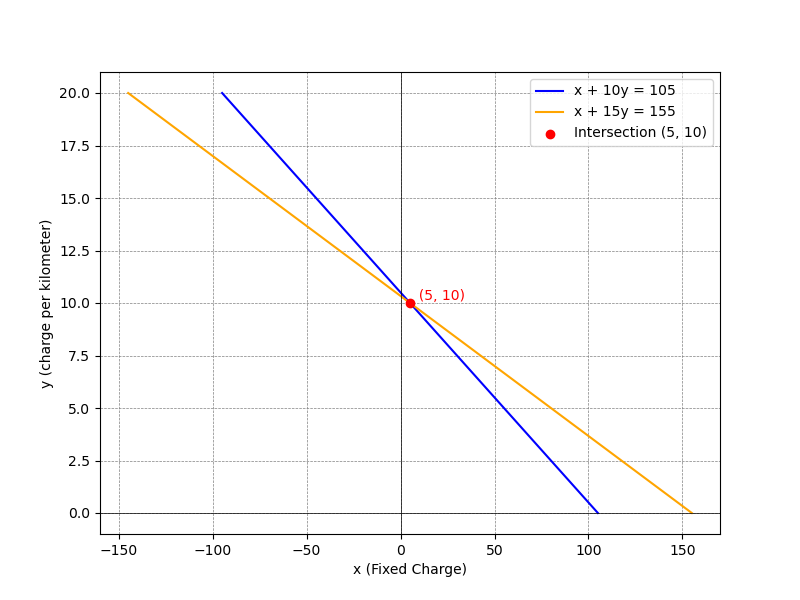
\includegraphics[width=0.7\linewidth]{Figure_1.png}
	\label{stemplot}
\end{figure}	
\end{frame}
\end{document}
